\documentclass[11pt,a4paper,oneside]{book}

% ==================== Packages ====================
\usepackage[T1]{fontenc}
\usepackage{lmodern}
\usepackage[a4paper,margin=1in,headheight=15pt]{geometry}
\usepackage{amsmath,amssymb,amsthm,mathtools,bm}
\usepackage{graphicx}
\usepackage{float}
\usepackage{booktabs,array}
\usepackage{enumitem}
\usepackage{xcolor}
\usepackage{listings}
\usepackage{fancyhdr}
\usepackage[hidelinks]{hyperref}
\usepackage[nameinlink,noabbrev]{cleveref}

% ==================== Environments ====================
\theoremstyle{remark}
\newtheorem{remark}{Remark}[chapter]

% ==================== Notation ====================
\newcommand{\R}{\mathbb{R}}
\newcommand{\X}{\mathbf X}
\newcommand{\y}{\mathbf y}
\newcommand{\I}{\mathbf I}
\newcommand{\bta}{\boldsymbol{\beta}}
\newcommand{\bhat}{\widehat{\boldsymbol{\beta}}}
\newcommand{\RSS}{\operatorname{RSS}}
\newcommand{\Var}{\operatorname{Var}}
\newcommand{\E}{\operatorname{E}}
\newcommand{\norm}[1]{\left\lVert #1\right\rVert_2}

\definecolor{navy}{RGB}{28,57,88}
\definecolor{lightblue}{RGB}{235,243,250}
\definecolor{codebg}{RGB}{247,248,250}
\definecolor{codegreen}{RGB}{35,110,65}
\definecolor{codepurple}{RGB}{115,55,140}

\lstdefinestyle{pythonstyle}{
  language=Python,
  basicstyle=\ttfamily\small,
  keywordstyle=\color{navy}\bfseries,
  commentstyle=\color{codegreen},
  stringstyle=\color{codepurple},
  backgroundcolor=\color{codebg},
  frame=single,
  rulecolor=\color{black!15},
  breaklines=true,
  showstringspaces=false,
  numbers=left,
  numberstyle=\tiny\color{black!50},
  xleftmargin=2em,
  framexleftmargin=1.5em
}
\lstset{style=pythonstyle}

\pagestyle{fancy}
\fancyhf{}
\fancyhead[L]{Ridge Regression}
\fancyhead[R]{Complete Learning Journey}
\fancyfoot[C]{\thepage}
\setlength{\parskip}{5pt}
\setlength{\parindent}{0pt}
\setlist[itemize]{leftmargin=1.5em}
\setlist[enumerate]{leftmargin=1.7em}

\title{\Huge\bfseries Ridge Regression\\[0.2em]}
\author{Noted by Md. Inzamamul Lohani\\
Software Engineering, IIT, DU}
\date{\today}

\begin{document}
\hypersetup{pageanchor=false}
\maketitle
\hypersetup{pageanchor=true}
\frontmatter

\tableofcontents
\mainmatter

% ==================================================
\chapter{The problem: why do we need Ridge Regression?}

\section{Start from what you already know}
In multiple linear regression, we describe the response using $p$ predictors:
\[
y_i=\beta_0+\beta_1x_{i1}+\beta_2x_{i2}+\cdots+\beta_px_{ip}
+\varepsilon_i.
\]
The coefficients describe how the predicted response changes when a
predictor changes, holding the other predictors fixed.

In matrix notation,
\[
\boxed{\y=\X\bta+\boldsymbol{\varepsilon}},
\]
where $\X$ contains the observed predictor values, $\bta$ contains the
unknown coefficients, and $\boldsymbol{\varepsilon}$ contains the errors.

For the moment, suppose the intercept has been handled separately or the
variables have been centered. OLS chooses coefficients by minimizing
\[
\boxed{\RSS(\bta)=\norm{\y-\X\bta}^2.}
\]
The familiar OLS estimator, when $\X'\X$ is invertible, is
\[
\boxed{\bhat_{\mathrm{OLS}}=(\X'\X)^{-1}\X'\y.}
\]

\section{The hidden issue: fitting the observed data is not the whole goal}
Imagine two models. Model A fits the training observations extremely closely,
but its coefficients change dramatically when a few observations change.
Model B has slightly more training error, but its coefficients and predictions
are much more stable.

Which model would you prefer for predicting new observations? Often, Model B.

OLS focuses on minimizing training RSS. It does not explicitly discourage
large or unstable coefficient estimates. When predictors contain overlapping
information, this can become a serious problem.

\section{The central question}
Ridge Regression asks:

\begin{quote}
Can we keep the model reasonably close to the observed data while discouraging
unnecessarily large coefficient values?
\end{quote}

This is the central idea of \textbf{regularization}. Ridge is a regularized
linear regression method. It adds a penalty to the OLS objective.

\section{What Ridge is not}
Ridge does not change the basic idea of a linear prediction. It does not
automatically discover a nonlinear relationship. It changes how the
coefficients are estimated by adding a preference for smaller coefficient
magnitudes.

\begin{remark}
A larger coefficient is not automatically bad. Ridge is useful when the
stability gained by shrinking coefficients is worth the small amount of
additional bias that shrinkage may introduce.
\end{remark}

% ==================================================
\chapter{Multicollinearity: when predictors are highly correlated}

\section{What does correlation between predictors mean?}
Suppose a dataset contains two predictors, $x_1$ and $x_2$. If knowing $x_1$
already tells us much of the value of $x_2$, the predictors are strongly
correlated. They carry similar information.

\begin{figure}[H]
\centering
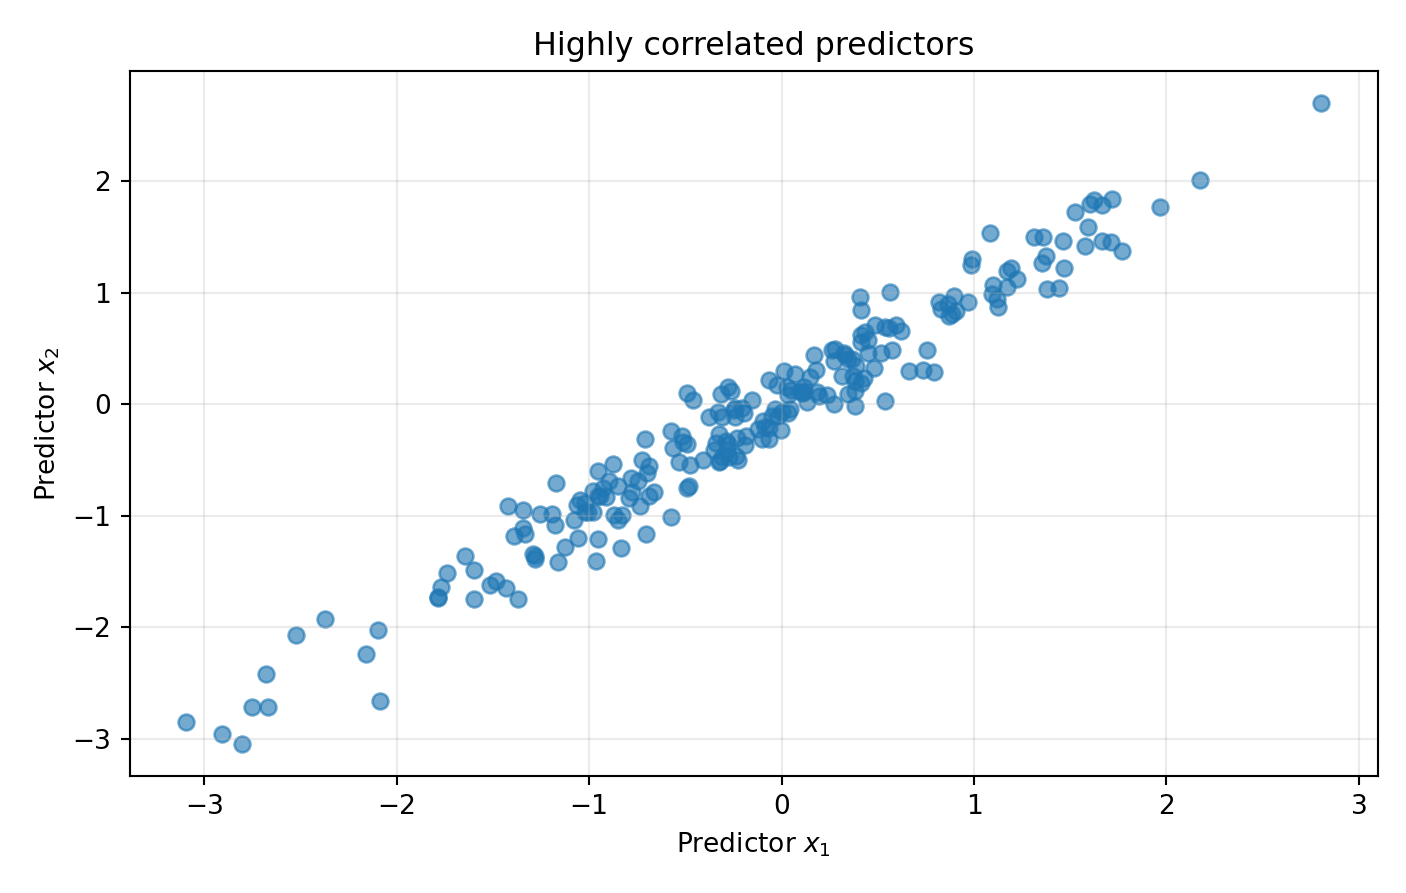
\includegraphics[width=.78\textwidth]{images/01_multicollinearity.png}
\caption{Illustration of two strongly correlated predictors. The points lie
close to a straight-line pattern, indicating that the predictors carry
overlapping information.}
\label{fig:multicollinearity}
\end{figure}

\section{Why does this create a problem for OLS?}
Consider the model
\[
y=\beta_0+\beta_1x_1+\beta_2x_2+\varepsilon.
\]
If $x_1$ and $x_2$ move together, it can be difficult to determine which
predictor deserves credit for a change in $y$.

For example, suppose study hours and time spent using a learning app are
strongly related. If both are included, the data may not contain enough
independent variation to estimate their separate effects precisely.

The model may still predict reasonably well, but the individual coefficients
can become unstable. A small change in the sample may produce a large change
in $\widehat\beta_1$ and $\widehat\beta_2$.

\section{The matrix explanation}
The OLS estimator contains $(\X'\X)^{-1}$. The matrix $\X'\X$ summarizes
relationships among the columns of $\X$. Strong dependence among columns
can make this matrix close to singular.

For a symmetric matrix, eigenvalues describe the amount of information in
different directions. If an eigenvalue is very small, inversion divides by
a very small number. Small disturbances can then be magnified.

\[
\X'\X=\mathbf Q\mathbf\Lambda\mathbf Q',
\qquad
\mathbf\Lambda=\operatorname{diag}(d_1,\ldots,d_p).
\]
The inverse contains $1/d_j$. If $d_j$ is tiny, the corresponding direction
can be highly sensitive.

\section{A simulation of coefficient instability}
The following illustration repeatedly samples similar data and estimates
the same two coefficients. OLS estimates spread widely because the
predictors are highly correlated. Ridge estimates are more concentrated.
The exact numerical pattern depends on the simulated data and penalty.

\begin{figure}[H]
\centering
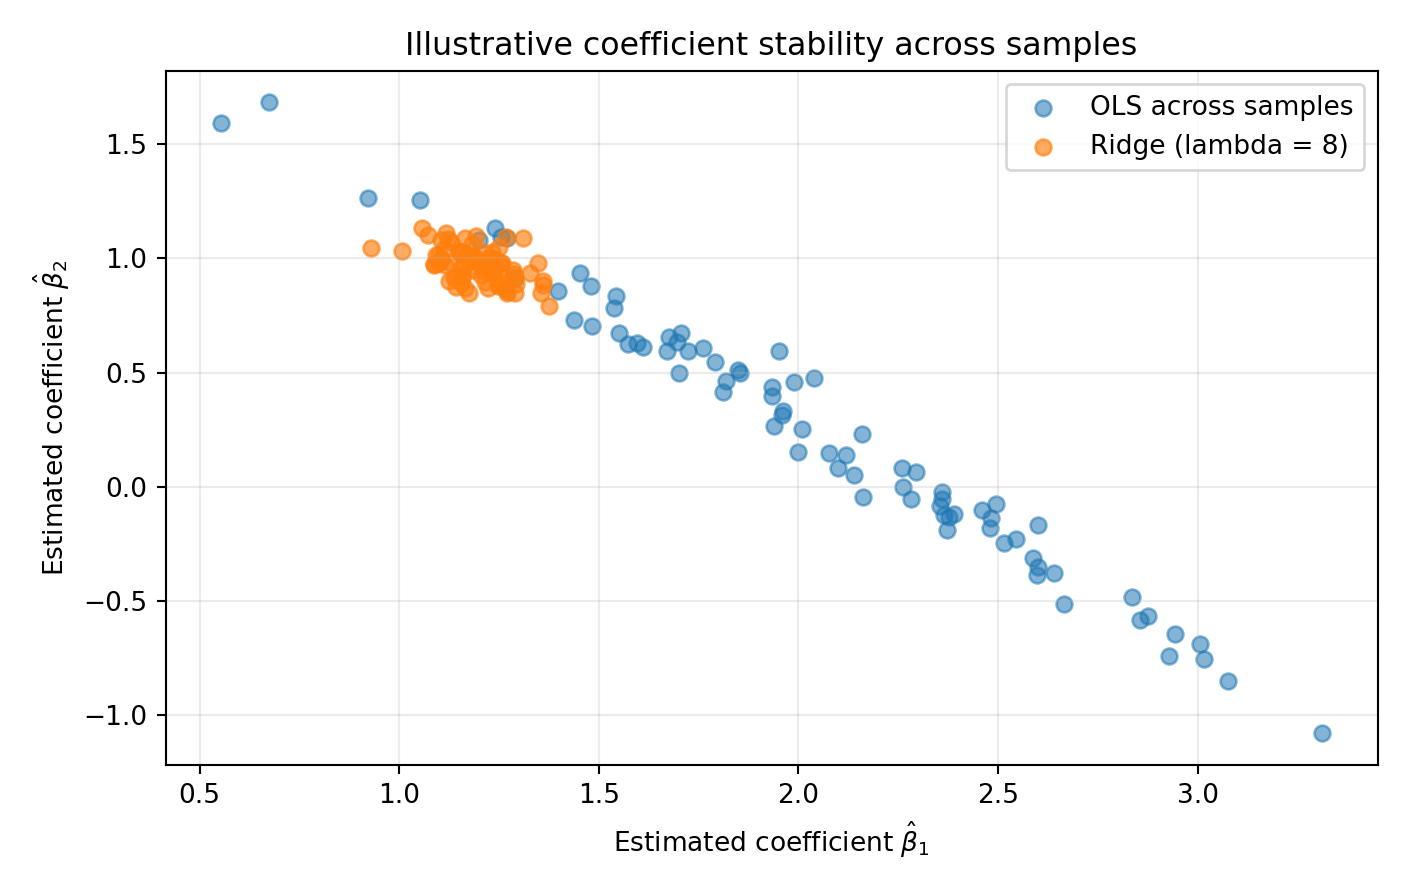
\includegraphics[width=.82\textwidth]{images/02_coefficient_stability.png}
\caption{Illustrative coefficient estimates across repeated samples.
Ridge shrinkage can reduce the variation of estimates when predictors are
highly correlated.}
\label{fig:stability}
\end{figure}

\begin{remark}
Multicollinearity is not the only reason to use Ridge. Ridge can also help
when the number of predictors is large relative to the number of observations,
or when prediction stability is important.
\end{remark}

% ==================================================
\chapter{Ridge intuition: how does Ridge address the problem?}

\section{The idea before the formula}
OLS says: choose coefficients that make residuals as small as possible.

Ridge says: choose coefficients that make residuals small, but also prefer
coefficients that are not unnecessarily large.

There are therefore two competing goals:
\begin{enumerate}
\item \textbf{Good fit:} predictions should remain close to observed responses.
\item \textbf{Controlled coefficients:} the coefficient vector should not
become excessively large.
\end{enumerate}

\section{What is shrinkage?}
Shrinkage means pulling coefficient estimates toward zero. Ridge usually
does not force coefficients to become exactly zero. Instead, it reduces
their magnitudes.

For example, an OLS estimate of $4.0$ might become a Ridge estimate of $3.2$.
An OLS estimate of $-2.0$ might become $-1.5$. These numbers are only
illustrative; actual shrinkage depends on the data and $\lambda$.

\section{Why can smaller coefficients help?}
When predictors are correlated, the model may use large positive and negative
coefficients to compensate for one another. Such a solution can fit the
training data but react strongly to small data changes.

Ridge discourages these large coefficient combinations. The result is often
a more stable model.

\section{A key distinction}
Ridge does not say ``make every coefficient as close to zero as possible''
without qualification. If that were the only goal, the all-zero vector would
win. Ridge balances coefficient size against fit. The penalty is only one
part of the objective.

% ==================================================
\chapter{Mathematical foundation: the Ridge cost function}

\section{Build the objective from the OLS objective}
The OLS objective is
\[
\RSS(\bta)=\norm{\y-\X\bta}^2.
\]
Ridge adds a penalty on squared coefficient magnitudes:
\[
\boxed{
J(\bta)=\norm{\y-\X\bta}^2+\lambda\norm{\bta}^2.
}
\]
Because
\[
\norm{\bta}^2=\bta'\bta
=\beta_1^2+\beta_2^2+\cdots+\beta_p^2,
\]
we can also write
\[
\boxed{
J(\bta)=\RSS(\bta)+
\lambda\sum_{j=1}^{p}\beta_j^2.
}
\]

\section{Understand each part}
\begin{itemize}
\item $\norm{\y-\X\bta}^2$ is the residual sum of squares. It measures
the mismatch between observed and fitted responses.
\item $\sum_j\beta_j^2$ measures the squared size of the coefficient vector.
\item $\lambda$ controls how strongly coefficient size is penalized.
\end{itemize}

\section{Why is it called an \texorpdfstring{$L_2$}{L2} penalty?}
The Euclidean length of a vector is
\[
\norm{\bta}=\sqrt{\beta_1^2+\cdots+\beta_p^2}.
\]
Ridge penalizes its square, $\norm{\bta}^2$. This is called an $L_2$
regularization penalty.

\section{The role of lambda}
The parameter $\lambda$ is nonnegative:
\[
\lambda\geq 0.
\]
When $\lambda=0$, the penalty disappears and the objective is OLS.
When $\lambda$ is positive, larger coefficient vectors receive a larger
penalty. As $\lambda$ increases, the optimization gives more importance
to keeping coefficients small.

\begin{center}
\begin{tabular}{@{}cl@{}}
\toprule
Penalty & Meaning\\
\midrule
$\lambda=0$ & OLS objective\\
Small $\lambda>0$ & Mild shrinkage\\
Moderate $\lambda$ & Stronger control of coefficient size\\
Very large $\lambda$ & Penalized coefficients approach zero\\
\bottomrule
\end{tabular}
\end{center}

\section{Why squares?}
Squaring makes the penalty smooth and differentiable. Large coefficients
are penalized more heavily than small ones. It also leads to a convex
quadratic optimization problem with a convenient closed-form solution.

% ==================================================
\chapter{Derivation: deriving the Ridge Regression estimator}

This chapter derives the estimator carefully. The purpose is to understand
where every term comes from.

\section{Step 1: write the objective}
Assume the intercept is not included in the penalized vector for now:
\[
J(\bta)=(\y-\X\bta)'(\y-\X\bta)+\lambda\bta'\bta.
\]

\section{Step 2: expand the residual term}
Use the identity $(A-B)'(A-B)=A'A-A'B-B'A+B'B$:
\[
\begin{aligned}
J(\bta)
&=\y'\y-\y'\X\bta-\bta'\X'\y
+\bta'\X'\X\bta+\lambda\bta'\bta.
\end{aligned}
\]
The two middle expressions are scalars and are transposes of one another.
A scalar equals its transpose, so
\[
\y'\X\bta=\bta'\X'\y.
\]
Therefore,
\[
J(\bta)=\y'\y-2\bta'\X'\y+
\bta'\X'\X\bta+\lambda\bta'\bta.
\]

\section{Step 3: combine the quadratic terms}
Since
\[
\bta'\X'\X\bta+\lambda\bta'\bta
=\bta'(\X'\X+\lambda\I_p)\bta,
\]
we obtain
\[
J(\bta)=\y'\y-2\bta'\X'\y+
\bta'(\X'\X+\lambda\I_p)\bta.
\]

\section{Step 4: differentiate}
We use two matrix-calculus identities:
\[
\frac{\partial(\mathbf c'\bta)}{\partial\bta}=\mathbf c,
\qquad
\frac{\partial(\bta'\mathbf A\bta)}{\partial\bta}
=(\mathbf A+\mathbf A')\bta.
\]
The matrix $\X'\X+\lambda\I_p$ is symmetric. Hence
\[
\frac{\partial J}{\partial\bta}
=-2\X'\y+2(\X'\X+\lambda\I_p)\bta.
\]

\section{Step 5: set the gradient equal to zero}
At the minimum, the gradient vanishes:
\[
-2\X'\y+2(\X'\X+\lambda\I_p)\bta=\mathbf 0.
\]
Divide by two:
\[
-\X'\y+(\X'\X+\lambda\I_p)\bta=\mathbf 0.
\]
Rearrange:
\[
(\X'\X+\lambda\I_p)\bta=\X'\y.
\]

\section{Step 6: solve for the coefficient vector}
For $\lambda>0$, the matrix $\X'\X+\lambda\I_p$ is invertible. Therefore,
\[
\boxed{
\bhat_{\mathrm{Ridge}}
=(\X'\X+\lambda\I_p)^{-1}\X'\y.
}
\]
This is the Ridge Regression estimator.

\section{Why does adding \texorpdfstring{$\lambda\I_p$}{lambda I\_p} help?}
The identity matrix is
\[
\I_p=
\begin{bmatrix}
1&0&\cdots&0\\
0&1&\cdots&0\\
\vdots&\vdots&\ddots&\vdots\\
0&0&\cdots&1
\end{bmatrix}.
\]
Thus, $\lambda\I_p$ adds $\lambda$ to every diagonal entry of $\X'\X$.

More importantly, if the eigenvalues of $\X'\X$ are
$d_1,\ldots,d_p$, the eigenvalues of
$\X'\X+\lambda\I_p$ are
\[
d_1+\lambda,\ldots,d_p+\lambda.
\]
Since $d_j\geq0$ and $\lambda>0$, every eigenvalue is positive. The matrix
is positive definite and therefore invertible.

\section{A proof of positive definiteness}
For any nonzero vector $\mathbf v$,
\[
\begin{aligned}
\mathbf v'(\X'\X+\lambda\I_p)\mathbf v
&=\mathbf v'\X'\X\mathbf v+\lambda\mathbf v'\mathbf v\\
&=(\X\mathbf v)'(\X\mathbf v)+\lambda\norm{\mathbf v}^2\\
&=\norm{\X\mathbf v}^2+\lambda\norm{\mathbf v}^2>0.
\end{aligned}
\]
This proves positive definiteness.

\section{Dimensions check}
If $\X$ has dimension $n\times p$, then
\[
\X'\X:(p\times n)(n\times p)=p\times p,
\]
and
\[
\X'\y:(p\times n)(n\times1)=p\times1.
\]
The inverse matrix is $p\times p$, so the final result is $p\times1$,
which is exactly the dimension of $\bta$.

\section{A tiny numerical example}
Suppose
\[
\X=\begin{bmatrix}1&1\\2&2\\3&3\end{bmatrix},
\qquad
\y=\begin{bmatrix}2\\4\\6\end{bmatrix}.
\]
Then
\[
\X'\X=\begin{bmatrix}14&14\\14&14\end{bmatrix},
\qquad
\X'\y=\begin{bmatrix}28\\28\end{bmatrix}.
\]
The columns of $\X$ are identical, so $\X'\X$ is singular. OLS cannot
uniquely decide how to split the total slope between the two identical
predictors.

For $\lambda>0$,
\[
\X'\X+\lambda\I_2=
\begin{bmatrix}14+\lambda&14\\14&14+\lambda\end{bmatrix}.
\]
Its determinant is
\[
(14+\lambda)^2-14^2=\lambda(28+\lambda)>0.
\]
So Ridge can solve the system. By symmetry, the two coefficients are equal:
\[
\widehat\beta_1=\widehat\beta_2=\frac{28}{28+2\lambda}.
\]
At $\lambda=1$, each coefficient is $28/30\approx0.933$. Their sum is
approximately $1.867$, close to the total slope of $2$ that reproduces
the response.

\begin{remark}
This example is intentionally extreme: the predictors are exactly identical.
It makes the matrix-stabilizing role of Ridge especially clear.
\end{remark}

% ==================================================
\chapter{Lambda: understanding the regularization parameter}

\section{Lambda controls the compromise}
The Ridge objective is
\[
J(\bta)=\RSS(\bta)+\lambda\norm{\bta}^2.
\]
Think of $\lambda$ as a volume control for the penalty term. A larger value
makes large coefficients more expensive.

\section{What happens at different values?}
\begin{itemize}
\item At $\lambda=0$, Ridge is OLS, assuming a unique OLS solution.
\item At a small positive value, coefficients are usually close to OLS.
\item At a larger value, coefficient magnitudes are reduced more strongly.
\item As $\lambda\to\infty$, penalized slope coefficients approach zero.
\end{itemize}

\section{Coefficient paths}
The following graph shows how estimated coefficients can change as lambda
moves across a range. It is generated from an illustrative dataset.

\begin{figure}[H]
\centering
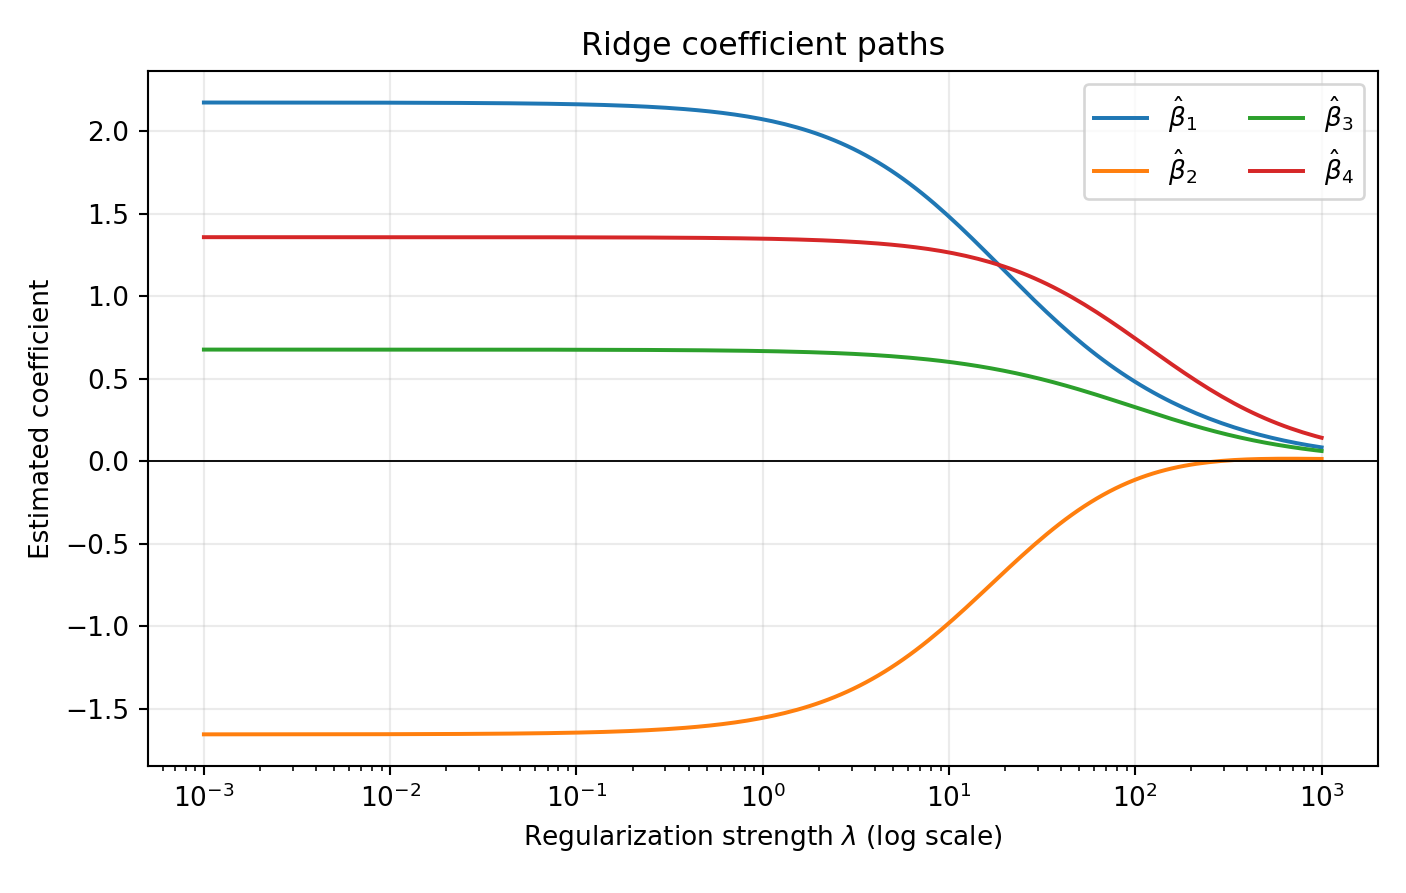
\includegraphics[width=.82\textwidth]{images/03_ridge_coefficient_paths.png}
\caption{Ridge coefficient paths. Coefficients generally move smoothly
toward zero as the penalty becomes stronger.}
\label{fig:paths}
\end{figure}

\section{Does larger lambda always mean a better model?}
No. A very large penalty can shrink useful coefficients too much. The model
may underfit. A very small penalty may fail to control instability. The
goal is to find a value that performs well on data not used to fit the model.

\begin{remark}
Do not choose lambda by minimizing training RSS. Training RSS generally
favors no penalty. Use validation data or cross-validation to estimate
performance on unseen observations.
\end{remark}

% ==================================================
\chapter{Geometrical intuition: Ridge using geometry}

\section{The constrained version}
Ridge can be written in two equivalent ways for suitable choices of the
penalty parameter and constraint size.

Penalized form:
\[
\min_{\bta}\RSS(\bta)+\lambda\norm{\bta}^2.
\]
Constrained form:
\[
\boxed{
\min_{\bta}\RSS(\bta)
\quad\text{subject to}\quad
\norm{\bta}^2\leq t.
}
\]
The constrained form says: find the best fit, but keep the coefficient vector
inside a circle (in two dimensions) or a sphere (in higher dimensions).

\section{Understand the contour picture}
An RSS contour connects coefficient combinations with the same RSS.
For a quadratic least-squares objective, these contours are ellipses.
The OLS estimate is at the center of the lowest reachable contour.

The Ridge constraint is an $L_2$ circle centered at the origin. Ridge chooses
the point where the smallest possible RSS contour touches the allowed region.

\begin{figure}[H]
\centering
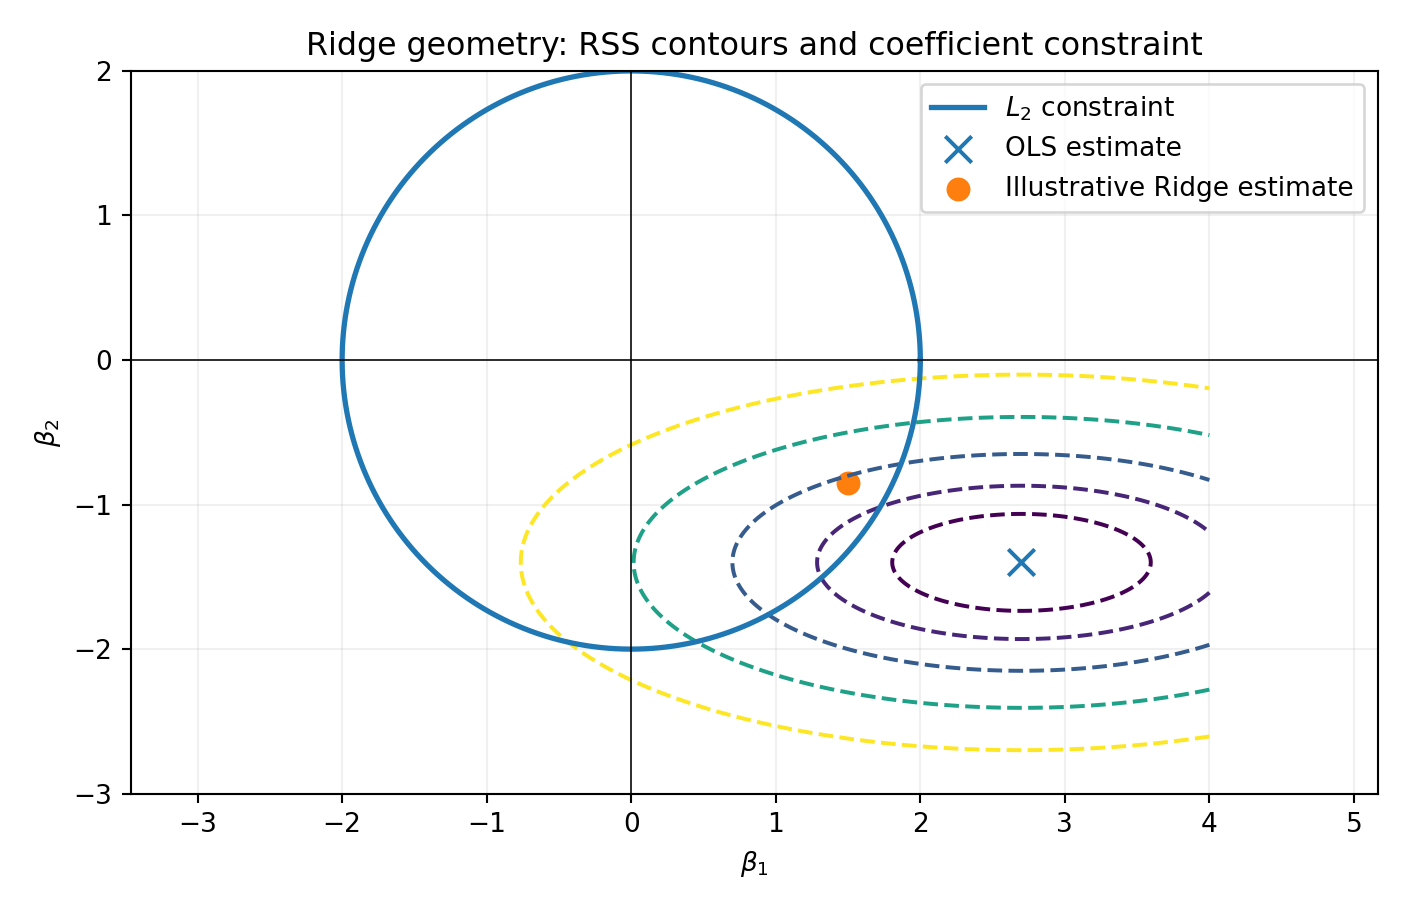
\includegraphics[width=.82\textwidth]{images/04_ridge_geometry.png}
\caption{Schematic geometric interpretation of Ridge. Dashed curves are
RSS contours; the circle is an $L_2$ constraint. The points are illustrative.}
\label{fig:geometry}
\end{figure}

\section{Why does Ridge shrink coefficients?}
The constraint limits the total squared coefficient size:
\[
\beta_1^2+\beta_2^2\leq t.
\]
If the OLS point lies outside the allowed circle, Ridge cannot choose it.
It must select a point closer to the origin. This is the geometric meaning
of shrinkage.

\section{A note about the intercept}
The usual intercept is not penalized. The circle applies to the slope
coefficients, not to the intercept. This is one reason centering predictors
and the response is convenient.

% ==================================================
\chapter{Bias--variance trade-off: why does Ridge introduce bias?}

\section{First, understand bias}
An estimator is unbiased if its expected value equals the true parameter:
\[
\E[\widehat\beta_j]=\beta_j.
\]
Ridge deliberately shrinks coefficients. Therefore, in general,
\[
\E[\widehat{\bta}_{\mathrm{Ridge}}]\neq\bta.
\]
This is why Ridge introduces bias.

\section{Why would we accept bias?}
Because the OLS estimator can have high variance. Variance measures how much
an estimate would change across repeated samples from the same process.

When predictors are highly correlated, OLS estimates can vary considerably
from one sample to another. Ridge often reduces this variation by shrinking
coefficients.

\section{Prediction error decomposition}
At a fixed input value, a standard squared prediction error decomposition is
\[
\begin{aligned}
\E[(Y_0-\widehat f(\mathbf x_0))^2]
={}&\Var(\widehat f(\mathbf x_0))\\
&+\operatorname{Bias}(\widehat f(\mathbf x_0))^2+\sigma^2.
\end{aligned}
\]
Here $\sigma^2$ is irreducible noise: variation in the response that the
predictors and model cannot explain.

Ridge may increase squared bias but reduce variance. If the variance
reduction is larger than the bias increase, total prediction error decreases.

\begin{figure}[H]
\centering
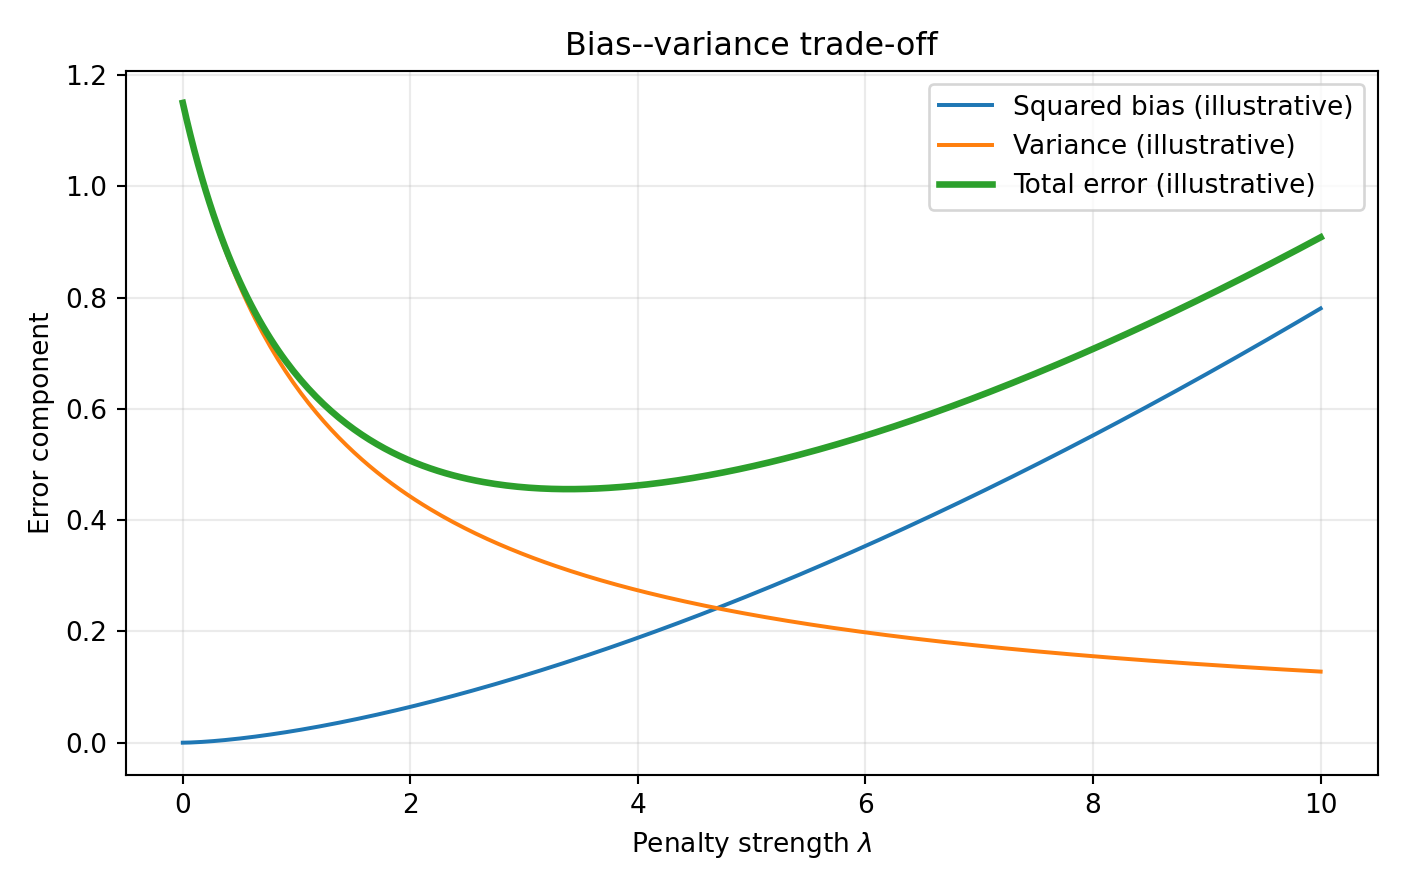
\includegraphics[width=.82\textwidth]{images/05_bias_variance.png}
\caption{Conceptual bias--variance curves. These curves are illustrative;
the exact shapes depend on the dataset and model.}
\label{fig:bv}
\end{figure}

\section{The key lesson}
The goal is not to make bias zero at all costs. The goal is good prediction
on new data. A slightly biased but stable estimator can outperform an
unbiased estimator with high variance.

% ==================================================
\chapter{Standardization: why must we scale features?}

\section{The problem with different units}
Suppose one predictor is measured in years, with values around $20$, while
another is measured in annual income, with values around $50{,}000$.
The numerical sizes of their coefficients can be very different simply
because the units are different.

Ridge penalizes coefficient magnitudes:
\[
\lambda(\beta_1^2+\cdots+\beta_p^2).
\]
If the predictor units change, the coefficients change too. Without scaling,
the penalty can treat predictors unfairly.

\section{Standardization formula}
For predictor $j$, calculate its training-set mean and standard deviation:
\[
\bar x_j=\frac{1}{n}\sum_{i=1}^n x_{ij},
\qquad
s_j=\sqrt{\frac{1}{n-1}\sum_{i=1}^n(x_{ij}-\bar x_j)^2}.
\]
Then transform each observation:
\[
\boxed{z_{ij}=\frac{x_{ij}-\bar x_j}{s_j}.}
\]
After standardization, each feature has mean approximately zero and sample
standard deviation one.

\begin{figure}[H]
\centering
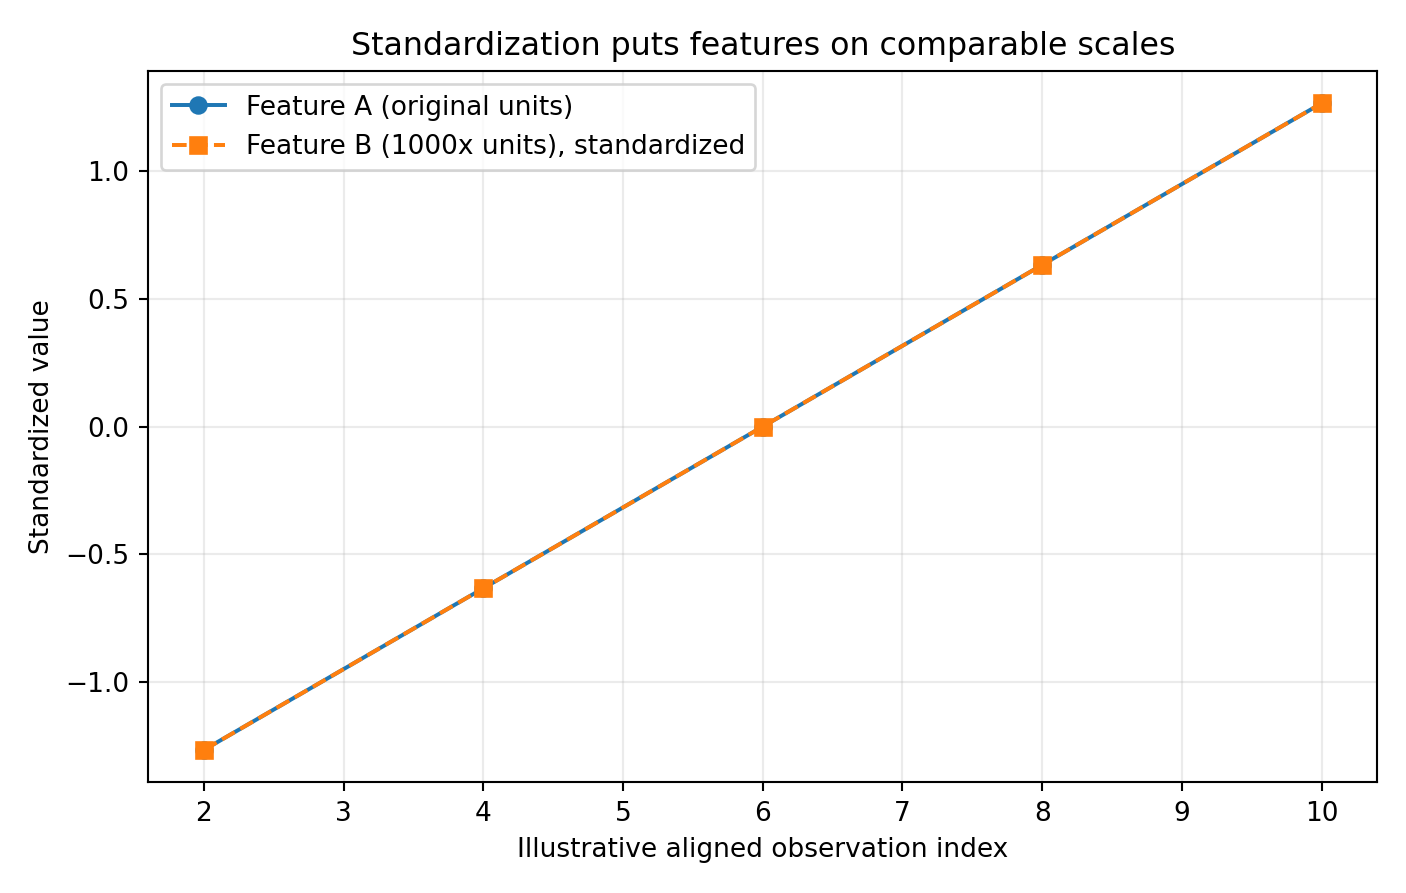
\includegraphics[width=.82\textwidth]{images/06_standardization.png}
\caption{Standardization makes feature scales comparable. Ridge is sensitive
to coefficient scale, so this preprocessing is usually important.}
\label{fig:scaling}
\end{figure}

\section{Why do we center the response?}
Centering the response makes the intercept easier to handle. In the standard
Ridge setup, the intercept is not penalized. After fitting centered data,
recover it using
\[
\boxed{\widehat\beta_0=\bar y-\sum_{j=1}^{p}\widehat\beta_j\bar x_j.}
\]

\section{A critical rule: avoid data leakage}
Calculate means and standard deviations using only the training portion of
the data. Apply those same values to validation and test data. If you use
the full dataset to calculate scaling statistics before splitting, information
from the held-out data leaks into the training process.

A machine-learning pipeline handles this correctly when used inside
cross-validation.

% ==================================================
\chapter{Practical implementation: Ridge Regression in Python}

\section{Install the libraries}
The example uses NumPy, pandas, Matplotlib, and scikit-learn:
\begin{lstlisting}
python -m pip install numpy pandas matplotlib scikit-learn
\end{lstlisting}

\section{Create an illustrative dataset}
We use a synthetic regression dataset so the example is reproducible and
does not depend on downloading a file.

\begin{lstlisting}
import numpy as np
from sklearn.datasets import make_regression
from sklearn.model_selection import train_test_split

X, y = make_regression(
    n_samples=500,
    n_features=8,
    n_informative=6,
    noise=18,
    random_state=42
)

X_train, X_test, y_train, y_test = train_test_split(
    X, y, test_size=0.2, random_state=42
)
\end{lstlisting}

\section{Why use a pipeline?}
A pipeline ensures that standardization is learned from the training data
inside each fold, then the Ridge model is fitted to the transformed data.
This helps prevent data leakage.

\begin{lstlisting}
from sklearn.pipeline import make_pipeline
from sklearn.preprocessing import StandardScaler
from sklearn.linear_model import Ridge

model = make_pipeline(
    StandardScaler(),
    Ridge(alpha=1.0)
)

model.fit(X_train, y_train)
predictions = model.predict(X_test)
\end{lstlisting}

In scikit-learn, the parameter is named \texttt{alpha}; it plays the role
of the Ridge penalty strength $\lambda$ in our mathematical notation.

\section{Evaluate predictions}
\begin{lstlisting}
from sklearn.metrics import (
    mean_squared_error,
    mean_absolute_error,
    r2_score
)

mse = mean_squared_error(y_test, predictions)
rmse = np.sqrt(mse)
mae = mean_absolute_error(y_test, predictions)
r2 = r2_score(y_test, predictions)

print("MSE:", mse)
print("RMSE:", rmse)
print("MAE:", mae)
print("R-squared:", r2)
\end{lstlisting}

\section{Understand the metrics}
\begin{itemize}
\item \textbf{MSE} averages squared prediction errors. Large errors receive
a particularly strong penalty.
\item \textbf{RMSE} is the square root of MSE and is expressed in the same
units as the response.
\item \textbf{MAE} averages absolute prediction errors and is less sensitive
to large individual errors than MSE.
\item \textbf{$R^2$} compares the model with a baseline that predicts the
training response mean. It can be negative on test data.
\end{itemize}

\section{Compare Ridge with OLS}
\begin{lstlisting}
from sklearn.linear_model import LinearRegression
from sklearn.pipeline import make_pipeline
from sklearn.preprocessing import StandardScaler

ols = make_pipeline(
    StandardScaler(),
    LinearRegression()
)

ridge = make_pipeline(
    StandardScaler(),
    Ridge(alpha=1.0)
)

ols.fit(X_train, y_train)
ridge.fit(X_train, y_train)

ols_pred = ols.predict(X_test)
ridge_pred = ridge.predict(X_test)

print("OLS RMSE:",
      mean_squared_error(y_test, ols_pred) ** 0.5)

print("Ridge RMSE:",
      mean_squared_error(y_test, ridge_pred) ** 0.5)
\end{lstlisting}

Do not assume Ridge must win. The test result depends on the data-generating
process and the penalty value.

% ==================================================
\chapter{Model evaluation: choosing the best lambda using cross-validation}

\section{Why do we need to choose lambda?}
Lambda controls the balance between fitting the data and shrinking
coefficients. A value that is too small may leave instability; a value that
is too large may underfit.

We need a principled way to compare candidate values. Cross-validation
estimates how well each candidate generalizes to data not used in its fit.

\section{\texorpdfstring{$K$}{K}-fold cross-validation}
The basic procedure is:
\begin{enumerate}
\item Divide the training data into $K$ approximately equal folds.
\item Choose one fold as validation data and fit on the other $K-1$ folds.
\item Evaluate predictions on the held-out fold.
\item Repeat until each fold has been used as validation data.
\item Average the validation errors for each candidate lambda.
\item Select the candidate with the best average validation score.
\end{enumerate}

\begin{figure}[H]
\centering
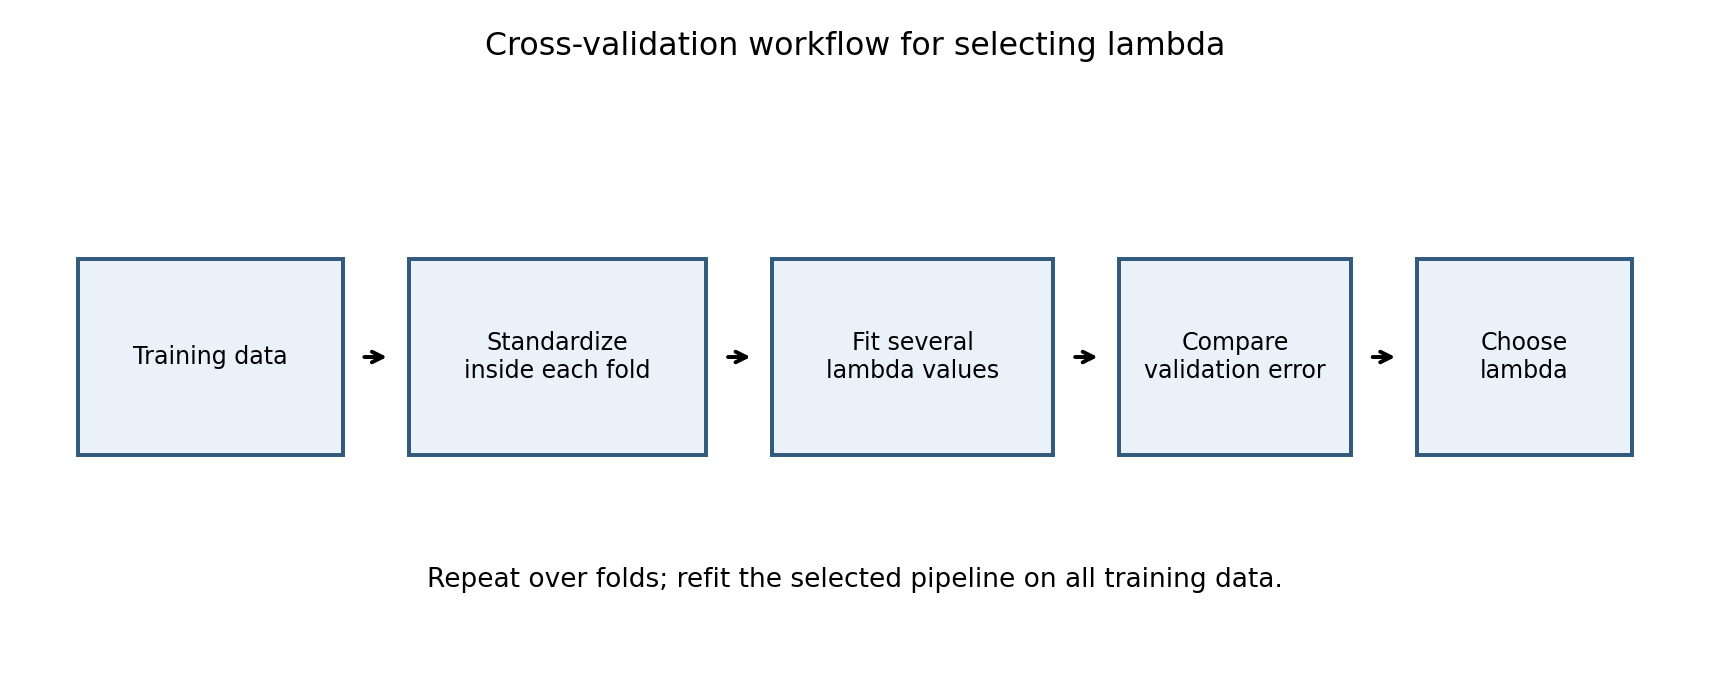
\includegraphics[width=.94\textwidth]{images/07_cross_validation_workflow.png}
\caption{A simplified workflow for selecting Ridge's penalty using
cross-validation.}
\label{fig:cvflow}
\end{figure}

\section{Cross-validation score}
For squared-error loss, a conceptual $K$-fold score is
\[
\operatorname{CV}(\lambda)=
\frac{1}{K}\sum_{k=1}^{K}
\left[
\frac{1}{n_k}\sum_{i\in\mathcal V_k}
(y_i-\widehat y_i^{(-k)}(\lambda))^2
\right].
\]
Here $\mathcal V_k$ is the validation fold and
$\widehat y_i^{(-k)}(\lambda)$ is the prediction from a model trained without
that fold.

\section{Use RidgeCV with a pipeline}
\begin{lstlisting}
import numpy as np
from sklearn.pipeline import make_pipeline
from sklearn.preprocessing import StandardScaler
from sklearn.linear_model import RidgeCV

alphas = np.logspace(-4, 4, 100)

ridge_cv = make_pipeline(
    StandardScaler(),
    RidgeCV(
        alphas=alphas,
        cv=5,
        scoring="neg_mean_squared_error"
    )
)

ridge_cv.fit(X_train, y_train)

ridge_step = ridge_cv.named_steps["ridgecv"]
print("Selected alpha:", ridge_step.alpha_)
\end{lstlisting}

The pipeline places the scaler inside the cross-validation process, so
each fold learns its own scaling parameters from its training portion.
The test set remains untouched during selection.

\section{Final evaluation on the test set}
After selecting lambda using training data and cross-validation, evaluate
the final fitted pipeline on the test set:
\begin{lstlisting}
from sklearn.metrics import mean_squared_error, r2_score

final_predictions = ridge_cv.predict(X_test)

test_rmse = np.sqrt(
    mean_squared_error(y_test, final_predictions)
)
test_r2 = r2_score(y_test, final_predictions)

print("Test RMSE:", test_rmse)
print("Test R-squared:", test_r2)
\end{lstlisting}

\begin{remark}
The test set should be used for final evaluation, not repeated tuning.
If you repeatedly inspect test performance and adjust the model, the test
set gradually becomes part of the model-selection process.
\end{remark}

% ==================================================
\chapter*{Final review: the complete Ridge story}
\addcontentsline{toc}{chapter}{Final review: the complete Ridge story}

The learning journey can be summarized in eleven connected steps:
\begin{enumerate}
\item OLS minimizes residual sum of squares.
\item Correlated predictors can make OLS coefficients unstable.
\item Ridge adds a preference for smaller coefficient magnitudes.
\item Its cost function combines RSS and an $L_2$ penalty.
\item Differentiation gives the modified normal equations.
\item Lambda controls the strength of shrinkage.
\item Geometry interprets Ridge as an RSS minimization under a coefficient constraint.
\item Ridge trades some bias for a possible reduction in variance.
\item Standardization makes the penalty fair across predictor scales.
\item Python pipelines implement scaling and Ridge together.
\item Cross-validation selects lambda; a separate test set evaluates final performance.
\end{enumerate}

The central estimator is
\[
\boxed{
\bhat_{\mathrm{Ridge}}
=(\X'\X+\lambda\I_p)^{-1}\X'\y
}
\]
when the intercept has been handled separately and all entries of the
coefficient vector are penalized.

For a standard model with an unpenalized intercept, center the predictors
and response or use a penalty matrix with zero in the intercept position.

\chapter*{Self-test}
\addcontentsline{toc}{chapter}{Self-test}
Try these questions without looking at the earlier chapters.

\begin{enumerate}
\item What does OLS minimize?
\item What is multicollinearity?
\item Why can multicollinearity make coefficient estimates unstable?
\item What does the Ridge penalty measure?
\item Why is $\lambda\I_p$ added to $\X'\X$?
\item What happens when $\lambda=0$?
\item What happens to penalized coefficients as $\lambda$ becomes very large?
\item Why does Ridge introduce bias?
\item How can reducing variance improve prediction?
\item Why should features be standardized?
\item Why must scaling be learned inside each cross-validation training fold?
\item Why should the test set be kept separate until final evaluation?
\end{enumerate}

\section*{Short answer guide}
\begin{enumerate}
\item Residual sum of squares.
\item Strong linear dependence among predictors.
\item The data struggle to distinguish their separate effects.
\item The squared Euclidean magnitude of the coefficient vector.
\item It shifts eigenvalues upward and makes the matrix positive definite for
positive lambda.
\item Ridge reduces to OLS when the OLS solution is uniquely defined.
\item They approach zero.
\item Shrinkage changes the expected coefficient estimates.
\item The reduction in variance can be larger than the increase in squared bias.
\item The penalty otherwise depends on arbitrary measurement units.
\item To prevent information leakage from validation observations.
\item To obtain an honest estimate of generalization performance.
\end{enumerate}

\backmatter
\chapter*{Where to go after Ridge}
After mastering these eleven topics, the next natural subjects are:
\begin{itemize}
\item the Bayesian interpretation of Ridge Regression;
\item singular value decomposition and Ridge shrinkage factors;
\item the Ridge hat matrix and effective degrees of freedom;
\item Lasso and Elastic Net;
\item Principal Component Regression.
\end{itemize}

\end{document}
